\subsection{Web services}
\label{sec:technology:web_services}

Для веб-сервисов в \LB предусмотрена своя платформа - \newline\sblox \cite{lb_web_services}. Сервисы \sblox предоставляют интерфейс для взаимодействия с базой \LB: будь то пользовательский интерфейс, инструменты для интеграций с данными либо сторонние приложения. К примеру, обычный сервис, который предоставляет данные для графиков или таблиц для отображения пользователю.

\sblox состоит из нескольких составляющих:

\begin{enumerate}
  \item \emph{Protobuf \cite{protobuf} services}. \http сервис, реагирующий на \http \post запрос. Запрос состоит из бинарного сообщения формата protobuf либо \json. Формат ответа такой же. В \sblox схема сообщений запроса и ответа должна соответствовать указанному формату protobuf протокола.
  \item \emph{Tabular data exchange (\tdx) services}. Доступны через \get, \post и \put запросы. \tdx сервис являются ключевым в загрузке и выгрузке данных из \LB базы в больших объемах. Как правило этот сервис используется для обновления большого количества информации с последними значениями (например, загрузке свежих данных о продажах, доставке и тп).
  \item \emph{Global Protobuf services} (рисунок \ref{fig:technology:web_services:global_protobuf}). Этот вид сервиса разделяет входящий запрос на несколько других в различные хранилища. Это полезно в тех случаях, когда \LB база данных распределена (находится в разных  \emph{workspaces}). Получив данные от каждого сервиса, этот сервис соединяет все ответы в один и возвращает результат. Таким образом, \emph{Global Protobuf service} реализует интерфейс для общения с клиентами.
  \item \emph{Proxy services}. Обычный proxy сервис. Могут представлять собой сервис для аутентификации пользователей.
  \item \emph{Custom services}. Реализуются как плагины к \sblox и представляют собой реализацию \java интерфейса. На самом деле, \tdx, Global Protobuf и Proxy сервисы реализованы как \emph{Custom service}, но уже встроены в платформу. Как правило, реализовывать свои сервисы не нужно, поскольку это усложняет разворачивание всей системы.
\end{enumerate}

\begin{figure}
	\centering
	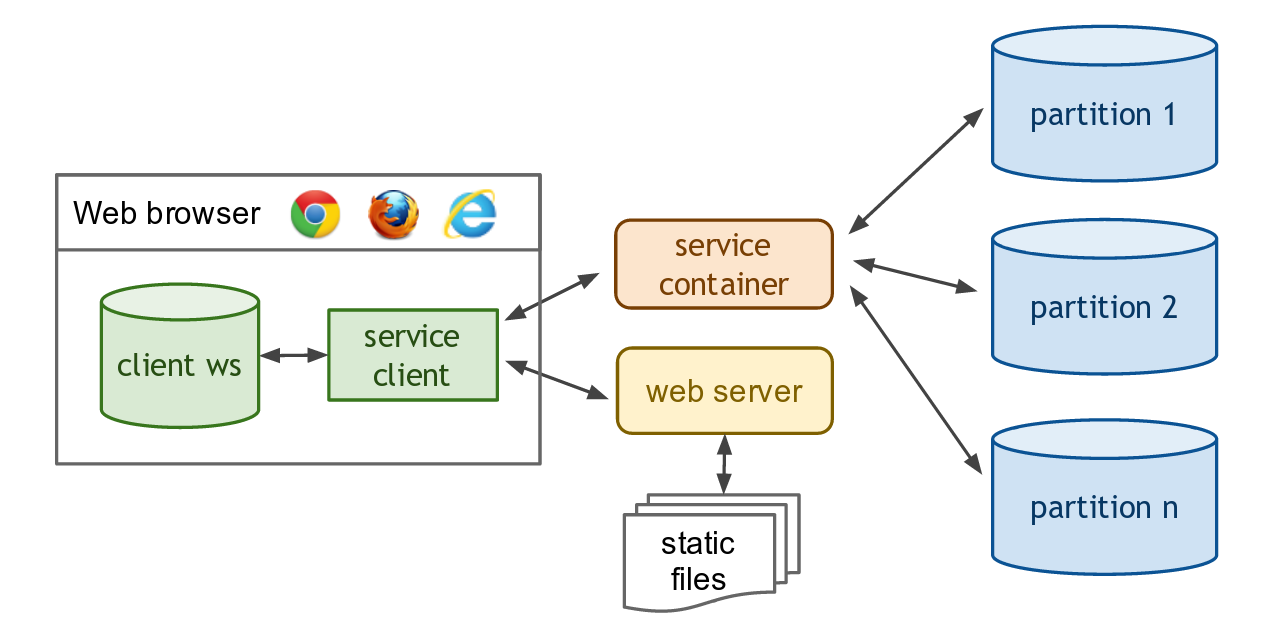
\includegraphics[scale=0.3]{global_protobuf.png}
	\caption{Распределение запросов с помощью Global Protobuf service \cite{lb_web_services}}
	\label{fig:technology:web_services:global_protobuf}
\end{figure}


\subsubsection{\tdx service}
\label{sec:technology:web_services:tdx}

Более подробно стоит остановиться именно на \tdx сервисе, поскольку в рамках оптимизации приложения из всех перечисленных видов предстояло немного настраивать именно этот сервис.

Настройка сервиса очень проста. Пусть у нас имеются следующие сущности:

\begin{lstlisting}[language=Prolog]
sku(x), sku_id(x:s) -> string(s).
store(x), store_id(x:s) -> string(s).
week(x), week_id(x:s) -> string(s).
\end{lstlisting}

А также целевая информация, которую необходимо сохранить:

\begin{lstlisting}[language=Prolog]
sales[x, y, z] = v -> sku(x), store(y), week(z), int(v).
\end{lstlisting}

Передача информации клиентом осуществляется через \lstinline{.csv} файлы:

\begin{lstlisting}[language=CSV]
SKU     | STORE       | WEEK | SALES
apples  | atlanta     | W1   | 10
oranges | atlanta     | W2   | 15
apples  | portland    | W1   | 20
oranges | portland    | W2   | 5
\end{lstlisting}

Задача \tdx сервиса - уметь загрузить данные из файла в предикат и выгрузить данные из предиката в файл. Для этого настраиваются три компонента:

\begin{enumerate}
  \item \emph{File definition (определение файла)}. Указывается структура файла - названия колонок, формат значений.
  \item \emph{File binding (привязка файла)}. Настраивается отображение колонок файла на ключи предиката. Эта настройка используется как для импорта, так и для экспорта.
  \item \emph{Service configuration}. Определение внешнего сервиса, вызов которого запустит импорт/экспорт данных.
\end{enumerate}

Если все объединить, то можно получить следующий пример настройки. \lstinline{file_definition} отвечает за \emph{File definition}, \lstinline{file_binding} - за \emph{File binding}, блок \lstinline{service_config} - за \emph{Service configuration}.

\begin{lstlisting}[language=Prolog]
block(`files) {
  alias_all(`lb:web:delim:schema),
  alias_all(`lb:web:delim:schema_abbr),
  alias_all(`lb:web:delim:binding),
  alias_all(`lb:web:delim:binding_abbr),

  clauses(`{
    file_definition_by_name["sales"] = fd,
    file_definition(fd) {
      file_delimiter[] = "|",
      column_headers[] = "SKU,STORE,WEEK,SALES",
      column_formats[] = "alphanum,alphanum,alphanum,integer"
    }.
  }),

  clauses(`{
    file_binding_by_name["sales"] = fb,
    file_binding(fb) {
      file_binding_definition_name[] = "sales",
      predicate_binding_by_name["measure:sales"] =
        predicate_binding(_) {
          predicate_binding_columns[] = "SKU,STORE,WEEK,SALES"
        }
    }.
  })
} <--.
\end{lstlisting}

\begin{lstlisting}[language=Prolog]
block(`service_config) {

  alias_all(`lb:web:config:service),
  alias_all(`lb:web:config:service_abbr),
  alias_all(`lb:web:config:delim),

  clauses(`{

    service_by_prefix["/sales"] = x,
    delim_service(x) {
      delim_file_binding[] = "sales"
    }.

  })

} <--.
\end{lstlisting}

Что же происходит в тот момент, когда вызывается сервис \lstinline{/sales}? Платформа сама создаст и установит в базу  \emph{дельта-предикаты}. С помощью таких предикатов также будет добавлено \logiql правило для целевого предиката в том случае, если в настройке определенного \tdx сервиса присутствуют дополнительные предикаты, с которыми нужно выполнить \join (проще говоря, отфильтровать входные данные. Например, по валидным сущностям). Такие сгенерированные правила могут оказать существенное влияние на оптимизацию приложения, поскольку стоит помнить о том, что платформа сама генерирует для них правила, а то, что неявно, часто забывается. Проблемы с \tdx сервисом, как следует из определения, часто возникают не в процессе пользования приложением конечными пользователями (имеется в виду время отклика системы на действия пользователя), а именно при обновлении данных (во время загрузки новых исторических данных, пересчете прогнозов и т.д.). То есть, оптимизации с \tdx носят \emph{оффлайн} характер.
